%\documentclass[a4paper]{article}
\documentclass[twocolumn]{article}

% graphics
\usepackage{graphicx}
\graphicspath{ {./images/} }

% Language and font encodings
\usepackage[english]{babel}

%\usepackage{biblatex}
%\addbibresource{refs.bib}

% *** CITATION PACKAGES ***
\usepackage{natbib}

\usepackage[utf8]{inputenc}
\usepackage[T1]{fontenc}
\usepackage{caption}
\captionsetup{font=footnotesize}

%% Sets page size and margins
% \usepackage[a4paper,top=3cm,bottom=2cm,left=3cm,right=3cm,marginparwidth=1.75cm]{geometry}
\usepackage[margin=.75in]{geometry}

\usepackage{float}
\floatstyle{plaintop}
\restylefloat{table}
\usepackage{appendix}
\setlength{\columnsep}{1cm}
\usepackage{multicol}
\usepackage{amsmath}
\usepackage[colorinlistoftodos]{todonotes}
\usepackage[colorlinks=true, allcolors=blue]{hyperref}
\usepackage{etoolbox}
\usepackage{lipsum}
\usepackage{booktabs}
\usepackage{changepage}
\usepackage{comment}
\usepackage{pdfpages}
\usepackage[labelfont = sc]{caption}
\DeclareCaptionFormat{mycaptionfont}{\fontsize{10}{10}\selectfont#1#2#3}
\captionsetup{format=mycaptionfont}
\usepackage{threeparttable}
\usepackage{verbatim}
\usepackage{multirow} 
\usepackage{float}

\AtBeginEnvironment{quote}{\par\singlespacing\small}
\usepackage{csquotes}


%%---------------------------------------------------------------
%%Begin Document 
\title{\Large \textbf{Rolling Stone: A Code Similarity Detection System}}
\author{\textbf{Albert (Yu) Jiang, Joe Mirza, Ricardo J\'enez} \\
\\
School of Information \\
University of California, Berkeley \\
\textit{\{yu.albert.jiang,mirza2020,rrj\}@ischool.berkeley.edu} \\
}
\date{}

\begin{document}
\maketitle


\begin{abstract}
Software plagiarism is a growing concern in academic and commercial software development environments. The state of the art in these NLP-PL systems (Natural Language Processing - Programming Languages) has not received as much attention and has not advanced as rapidly as it has for more conventional NLP tasks. Our contribution in this paper is developing an NLP system that performs code similarity detection on software code using state of the art deep learning architectures. This system allows the detection of similar code programs (not just snippets) and determines if there is sufficient similarity between code examples to warrant further review for plagiarism. Our objective was to outperform the industry-standard similarity detection system, named MOSS (“Measure Of Software Similarity”) which uses text fingerprinting\cite{schleimer} to identify software similarity. We appear to have achieved this for a large labeled corpus of C programming assignments.
\end{abstract}


\section{\large Introduction}
In many universities, there is an increased incidence of plagiarism in code implemented by students in programming assignments \cite{bowyer}. Similarly, in industry, commercial code is frequently “infected” by code snippets taken from the open-source or on popular sites like StackOverflow (SO), leading to liabilities for companies who have made unauthorized use of that code.

Additionally, copy and paste code leads to more brittle code bases. Detecting similar code fragments that are swept up into common functions or classes would significantly reduce code complexity. “Recent studies have shown that developers use SO snippets in their software projects, regardless of maintainability, security, and licensing implications...”. \cite{baltes}.

The most frequently used software plagiarism detection tool is named MOSS (“Measure Of Software Similarity” \cite{schleimer}), developed at UC Berkeley by Alex Aiken, et al. based upon the paper\cite{schleimer}. MOSS has been in use for over 20 years and is still the gold standard. Given the advances in NLP and Deep Learning, we were curious to see if we might be able to develop a deep learning plagiarism detector that was better than MOSS.

The advent of attention-oriented architectures such as Transformers \cite{viswani} and the language models they've enabled, such as BERT\cite{devlin} and T5\cite{raffel}, would seem to provide an opportunity to advance the state of the art in this area. Programming Language (PL) variants, such as CodeBERT, trained on large code corpora, seem even more promising. 



\section{\large Data Acquisition}

There are several factors to consider when determining if two code files, or parts of those files, are similar and whether that similarity is potentially the result of plagiarism. Neither syntactic nor semantic similarity alone is sufficient to conclude that plagiarism has occurred. Two pieces of code can be semantically quite similar (i.e. they solve the same problem), but arrive at the solution using different approaches (e.g. a while loop vs a for loop for iteration). Syntactic similarity, where the code is the same word for word, may not be flagged as being copied,  if variable names are modified or functions are ordered differently. 


Given this, we decided that more stringent similarity thresholds were needed in order to make a plagiarism determination between two pieces of code. It lies between pure syntactic similarity and semantic similarity. We looked at work done by Oscar Karnalim, et. al. \cite{karnalim2019}, to provide some of the needed context for this task. By leveraging a labeled plagiarization dataset, we can attempt to assess both syntactic and semantic similarity and perhaps get insights into intent to plagiarize as well. 

In searching for a robust plagiarism dataset, we looked at several options, including datasets for code generation from text (CodeXGlue) which has several different datasets from CodeBert trained with a variety of coding tasks\cite{lu} as well as StatQC \cite{yin} which looked at Stack Overflow code snippets. We felt that we needed to better control the experience and align it with actual software practices in universities or commercial settings, where we could confirm plagiarism with the code authors as in the dataset compiled by Ljubovic \cite{ljubovic}. We will go into more detail below about the options and concerns for each case. (See Appendix for an overview of the datasets we chose from in Table~\ref{table:datasetoptions}.)


\subsection{\normalsize Data Sets}

Our primary dataset is Programming Homework Dataset for Plagiarism Detection
Dataset \cite{ljubovic}. It is used to examine how student programming styles and IDE usage differs between students who plagiarize their homework and those who do not. Ljubovic uses code from an introductory programming class with $\sim500$ students per class. When determining whether a particular assignment has been plagiarized, they not only look at code similarity but also offer students the opportunity to refute a determination of plagiarism. Those students who do not mount a defense are determined to have plagiarized their code.

\begin{comment}
Other datasets we considered are in Table (see Table \ref{table:datasetoptions}  on page \pageref{table:datasetoptions})


\begin{itemize}
  \item IR-Plag data set (Personal communication with author Oscar Karnalim)\cite{karnalim2019} which looks at actual programming exercises by students.  It is substantially smaller than the Ljubovic dataset \cite{ljubovic}, but looks at canonical cases of plagiarization.
  \item StaQC: A Systematically Mined Question-Code Dataset from Stack Overflow \cite{yao}.StaQC (Stack Overflow Question-Code pairs) is the largest dataset to date of around 148K Python and 120K SQL domain question-code pairs, which are automatically mined from Stack Overflow using a Bi-View Hierarchical Neural Network, as described in the paper. This dataset, like the Conala dataset that follows, was primarily designed to allow code generation from text.
  \item The Conala \cite{yin} dataset was created as a challenge designed to test systems for generating program snippets from natural language. For example, if the input is `sort list x in reverse order`, then the system would be required to output `x.sort(reverse=True)` in Python. The dataset is automatically filtered, then curated by annotators, split into 2,379 training and 500 test examples. Additionally, they also provide a large automatically-mined dataset with 600k examples and links to other similar datasets. These datasets can be used for the CoNaLa challenge or for any other research on the intersection of code and natural language.
\end{itemize}
\end{comment}


\begin{comment}
\subsection{\normalsize Data Set Under Consideration}
\end{comment}
\subsection{\normalsize Data Set Preparation}



The first challenge with this task is determining similarity and the second is determining plagiarism, which implies intent. To do this we augmented the Homework Dataset \cite{ljubovic} (which contains the binary plagiarization label) with MOSS's similarity measures. We did this by running each source code pair for a particular assignment through MOSS, which provided us with MOSS's evaluation of percent similarity between each file pair and the number of lines that were similar. This provided us with a MOSS baseline for each document pair. 

\begin{comment}
\sWe may build our  NLP system on top of transformers like BERT and code-specific transformers like CodeBerta (perhaps even CODEX if we gain access). The goal will be to use these systems trained on datasets (#1, #2)  to identify similar code snippets above five lines from the SO-related dataset (#3,4,5).

Once we have Rolling Stone functioning, we intend to compare its performance against specific systems designed to defeat plagiarism detection, such as Mossad (“Mossad: Defeating Software Plagiarism Detection” \cite{devore-mcdonald}) and validate whether our system can do better than MOSS when presented with sophisticated tools built to evade plagiarism detection.
\end{comment}

MOSS produces output of the top N pairs that are similar in HTML files that we download. We set N = 1000 for each assignment. We then processed these HTML files and joined them with the plagiarism labels from the Homework dataset. We generated training and test sets from these top 1000 pairs for each assignment and there were between sixteen and twenty assignments per year. These training/test examples are put in csv files with each line having percent similarity, both sources from the files, the filename identifiers, the percent similarity, and a label indicating whether or not the source code pairs were plagiarized.  The source code from each file ranges between 79 bytes up to 11K bytes. Our training and test set reflected an 80/20 split of the 17,280 samples. We viewed this as sufficient data to fine-tune these pre-trained models and determine if our model was better than MOSS at identifying plagiarism. 


\section{\large Initial Approach}

Before creating our models, we attempted to replicate one of the small number of papers in this space from Karnalim et al. \cite{karnalim2019}. They had a relatively small Java dataset, which contained 105 non-plagiarized files and 355 plagiarized ones, and used a Vector Space Model (VSM) and Language Model (LM) to predict plagiarism. 

For the VSM techniques, we vectorized each file's token count with respect to the collection's token count, then compared the vector of each original code file to the vectors of its related files that were either plagiarized or not plagiarized to get cosine similarity values. For the LM techniques, we compared the token count of each original code file against the token count of each of its related files and of the entire collection to get similarity values.

For both VSM and LM, we used the similarity measures that Karnalim et al. used. We then ranked the files by similarity and then applied mean average precision (mAP) to the file rankings. On balance, our mAP values were similar to Karnalim et al.

We then attempted to use the VSM and LM based techniques on a portion of our main dataset. Although the VSM based techniques consistently outperformed LM based techniques, neither technique attained mAP scores significantly greater than 0.5 on any of the variants of each method we applied.  We concluded these techniques did not perform well enough to pursue further.  

\begin{table*}[ht]
\centering
\captionsetup{font=small}
\caption{\textsc{Moss As Measure Of Plagiarism Vs.Cosine Similarity Of Embeddings}}
\fontsize{20}{24}\selectfont 
\label{table:mosscomparisons}
\resizebox{\textwidth}{!}{%
\begin{tabular}{llllll}
\toprule
\textbf{Model}& \parbox{15cm}{\textbf{Experiment Details}}  & \textbf{Accuracy} & \textbf{Precision}  & \textbf{Recall}  & \textbf{F1-Score}  \\ \midrule
\parbox{7cm}{MOSS} & \parbox{15cm}{Code pairs, similarity, 50 setting for code common block. Evaluate at similarity above 73.1 pcnt to get max accuracy} & \parbox{3cm}{\textbf{0.6970}} & \parbox{3cm}{\textbf{0.6840}} & \parbox{3cm}{\textbf{0.7325}}  & \parbox{3cm}{\textbf{0.7074}}\\
\midrule
\hline
\parbox{7cm}{BERT}  & \parbox{15cm}{bert-base-uncased, average embeddings over 256 Tokens from sentence-transformer, cosine sim = 0.9674 and above, max pooling}  & \parbox{3cm}{0.6519} & \parbox{3cm}{0.6505} & \parbox{3cm}{0.6566}  & \parbox{3cm}{0.6536}\\
\midrule 
\parbox{7cm}{CodeBERT}   & \parbox{15cm}{microsoft/codebert-base, average embeddings over 256 Tokens from sentence-transformer, cosine sim = 0.9747 and above, max pooling} & \parbox{3cm}{0.6603} & \parbox{3cm}{0.6796} & \parbox{3cm}{0.6066}  & \parbox{3cm}{0.6410}\\
\midrule 
\parbox{7cm}{LongFormer}  & \parbox{15cm}{allenai/longformer-base-4096,2K tokens, from sentence transformer, cosine sim 0.9367 and above, max pooling}  & \parbox{3cm}{ 0.6307}  & \parbox{3cm}{0.6164} & \parbox{3cm}{0.6922}  & \parbox{3cm}{0.6521}\\
\midrule 
\parbox{7cm}{T5Large}   & \parbox{15cm}{sentence-transformers/sentence-t5-large, 2K tokens, from sentence transformers,mean pooling, min similarity 0.29, mean pooling} & \parbox{3cm}{0.5619} & \parbox{3cm}{0.5712} & \parbox{3cm}{0.4967}  & \parbox{3cm}{0.5313}\\
\midrule
\addlinespace[0.5em]

\end{tabular}%
}
\end{table*}

\section{\large Main Approach}

As mentioned in section 2, we generated a dataset that had MOSS scores along with annotation/labels from the Homework Plagiarization dataset. This provided us with a MOSS baseline for all of our experiments. We started by applying simple techniques such as Sentence Embeddings and Cosine Similarity to assess similarity for plagiarized and unplagiarized code pairs. 

We then compared these results with more specifically trained models. One significant challenge we encountered was that models like BERT and CodeBERT have token limits of 512, while many of the code files would require 10x that many tokens or more to represent in their entirety. That led us to experiment with models capable of longer token inputs, such as LongFormer and BigBird. 

\subsection{\normalsize Experimentation with Embeddings}

To start, we encoded each document using BERT, CodeBERT, LongFormer, and T5Large as-is (without fine tuning on our task) and applied either max or mean pooling to get a single vector for each document. Next, we calculated cosine similarity for each file pair using those embeddings. We then plotted Accuracy, Precision, Recall and F1 against ascending values of those similarity scores. In Table \ref{table:mosscomparisons}  on page \pageref{table:mosscomparisons}, we show the performance of these models along these metrics, with MOSS performance as our base case. In that table, the value maximized is accuracy. At the similarity that maximizes accuracy for each model, the other three metrics are provided. (The data-set is balanced between plagiarized and not plagiarized.)

MOSS outperforms these simple, embeddings-based models across all four metrics. At 73.1\% similarity, MOSS sees its maximum accuracy of 69.7\%. We were surprised that LongFormer and T5Large performed so poorly relative to BERT and CodeBERT. We had expected those models' larger maximum input lengths to capture more signal and result in outperformance. 


\begin{table*}[ht]
\centering
\captionsetup{font=small}
\caption{\textsc{Trained Model Performance}}
\fontsize{20}{24}\selectfont 
\label{table:trainedmodels2}
\resizebox{\textwidth}{!}{%
\begin{tabular}{llllll}
\toprule
\textbf{Model}   & \parbox{15cm}{Experiment Details} & \textbf{Accuracy} & \textbf{Precision}  & \textbf{Recall}  & \textbf{F1-Score}  \\ \midrule
\parbox{7cm}{MOSS} & \parbox{15cm}{Code pairs, similarity, 50 setting for code common block. Evaluate at similarity above 73.1 \% to get max accuracy} & \parbox{3cm}{0.6970} & \parbox{3cm}{0.6840} & \parbox{3cm}{0.7325}  & \parbox{3cm}{0.7074}\\
\midrule
\hline
\parbox{7cm}{BERT}   & \parbox{15cm}{bert-base-uncased,512 tokens max ,learning rate 1e-5} & \parbox{3cm}{0.7833} & \parbox{3cm}{0.8032} & \parbox{3cm}{0.7505}  & \parbox{3cm}{0.7760}\\
\midrule 
\parbox{7cm}{BERT - Chinese Model}   & \parbox{15cm}{bert-base-chinese,512 tokens max,learning rate 1e-5}  & \parbox{3cm}{0.7676} & \parbox{3cm}{0.7460} & \parbox{3cm}{0.8114}  & \parbox{3cm}{0.7774}\\
\midrule 
\parbox{7cm}{CodeBERT}  & \parbox{15cm}{codebert-base,512 tokens, learning rate= 1e-5} & \parbox{3cm}{0.7845} & \parbox{3cm}{0.8144} & \parbox{3cm}{0.7367}   & \parbox{3cm}{0.7737}\\
\midrule 
\parbox{7cm}{BigBird 1K}  & \parbox{15cm}{google/bigbird-roberta-base, 1K tokens, attention_type original_full, learning rate 1e-5}  & \parbox{3cm}{0.7369} & \parbox{3cm}{0.6992} & \parbox{3cm}{0.8318}  & \parbox{3cm}{0.7597}\\
\midrule 
\parbox{7cm}{BigBird 2K}  & \parbox{15cm}{google/bigbird-roberta-base, 2K tokens,learning rate 1e-5)}  & \parbox{3cm}{0.7585} & \parbox{3cm}{0.8369} & \parbox{3cm}{0.6421}  & \parbox{3cm}{0.7261}\\
\midrule 
\parbox{7cm}{Longformer 4K}  & \parbox{15cm}{allenai/longformer-base-4096, 4K tokens, learning rate 1e-5} & \parbox{3cm}{0.7140} & \parbox{3cm}{0.8322} & \parbox{3cm}{0.5361}  & \parbox{3cm}{0.6521}\\
\bottomrule
\addlinespace[0.5em]

\end{tabular}%
}
\end{table*}

\subsection{\normalsize Experimentation with Model Training}

Our next step was to fine-tune these transformer-based models on our plagiarism classification task. We started with BERT, CodeBERT, the BERT Chinese model, BigBird 1K and 2K as well as Longformer 4K. This work is summarized in Table~\ref{table:trainedmodels2} on page \pageref{table:trainedmodels2}. We trained each of our models for 4 Epochs and used an 11K/3.5K/3.5K split for training, validation and test  (after randomly over sampling the minority class we had 21K/7K/7K). 
We used a BERT based Tokenizer (Roberta in the case of CodeBERT), and Models based upon Trainers for SequenceClassification. 

All of the trained models outperformed MOSS by Accuracy and all of the models except Longformer 4K outperformed MOSS by F1-Score. So training is effective. BERT and CodeBERT outperformed the models with larger maximum input lengths (BigBird 1K, 2K and Longformer 4K). Strangely, the BERT Chinese model performed about as well as BERT and CodeBERT. Why this was the case provided us with a useful insight on the importance of tokenization methods, which we'll explore in the next section. 


\subsection{\normalsize Experimentation with Whole Word Masking}

As noted in the last section, the Chinese BERT model had the highest F1-Score. Why would a model trained on Chinese perform so well? We learned that the Chinese BERT model uses whole word masking, while BERT models use wordpiece tokenization, which can split each word into token parts (e.g. "surfing" becomes "surf" and "ing"). Furthermore, we know that normal BERT models only mask on a token level. This method can help reduce the size of the vocabulary, while increasing its expressiveness.  However, we hypothesized that it does not perform as well when dealing with programming language code elements. To deal with such documents, masking each code element in its entirety instead of masking tokenized parts helps retain the integrity of the vocabulary. To address this, we trained on an uncased BERT Large model that uses whole word masking. This model produced our best results yet, beating the BERT model trained on Chinese. This is summarized in Table~\ref{table:trainedmodels3} on page \pageref{table:trainedmodels3}. While whole word masking did not play a part in our best model, understanding why the Chinese BERT model performed so well provided us with a better understanding of the importance of the right choice of tokenization methods. 


\begin{table*}[ht]
\centering
\captionsetup{font=small}
\caption{\textsc{Trained Model Performance - Whole Word Masking}}
\fontsize{20}{24}\selectfont 
\label{table:trainedmodels3}
\resizebox{\textwidth}{!}{%
\begin{tabular}{llllll}
\toprule
\textbf{Model}   & \parbox{15cm}{Experiment Details} & \textbf{Accuracy} & \textbf{Precision}  & \textbf{Recall}  & \textbf{F1-Score}  \\ \midrule
\parbox{7cm}{MOSS} & \parbox{15cm}{Code pairs, similarity, 50 setting for code common block. Evaluate at similarity above 73.1 \% to get max accuracy} & \parbox{3cm}{0.6970} & \parbox{3cm}{0.6840} & \parbox{3cm}{0.7325}  & \parbox{3cm}{0.7074}\\
\midrule
\hline
\parbox{7cm}{BERT}   & \parbox{15cm}{bert-base-uncased,512 tokens max ,learning rate 1e-5} & \parbox{3cm}{0.7833} & \parbox{3cm}{0.8032} & \parbox{3cm}{0.7505}  & \parbox{3cm}{0.7760}\\
\midrule 
\parbox{7cm}{BERT - Chinese Model}   & \parbox{15cm}{bert-base-chinese,512 tokens max,learning rate 1e-5}  & \parbox{3cm}{0.7676} & \parbox{3cm}{0.7460} & \parbox{3cm}{\textbf{0.8114}}  & \parbox{3cm}{0.7774}\\
\midrule 
\parbox{7cm}{BERT w/Whole Word}  & \parbox{15cm}{bert-large-uncased-whole-word-masking, 512 tokens,learning rate 1e-5} & \parbox{3cm}{\textbf{0.8194}} & \parbox{3cm}{\textbf{0.8809}} & \parbox{3cm}{0.7386}  & \parbox{3cm}{\textbf{0.8035}}\\
\midrule 
\parbox{7cm}{CodeBERT}  & \parbox{15cm}{codebert-base,512 tokens, learning rate= 1e-5} & \parbox{3cm}{0.7845} & \parbox{3cm}{0.8144} & \parbox{3cm}{0.7367}   & \parbox{3cm}{0.7737}\\
\bottomrule
\addlinespace[0.5em]

\end{tabular}%
}
\end{table*}

\subsection{\normalsize Experimentation with Preprocessing}


To attempt to further improve our models,  we analyzed some of the false negatives and false positives of our best models. In the course of this analysis, we observed that whitespace and comments represented a large fraction of the tokens. We suspected they had little predictive power and, given the maximum input limits on our best models (512 tokens), these tokens were \textit{displacing} tokens that might actually possess some predictive power. 

To address this, we used ANTLR, a customizable parsing tool we had used to preprocess the code files in the VSM/LM models mentioned previously, to ignore whitespace and comments and lower case all tokens. When our models were rerun on the code files with this preprocessing, we saw a noticeable improvement to the BERT Large model that uses whole word masking. CodeBERT performed even better, despite not using whole word masking. In fact, the CodeBERT model with ANTLR preprocessing was our best overall model.  This is summarized in Table~\ref{table:trainedmodels4} on page \pageref{table:trainedmodels4}, and an example of the before and after tokens can be seen in Figure~\ref{fig:beforeandafterANTLR} in the Appendix.


\begin{table*}[ht]
\centering
\captionsetup{font=small}
\caption{\textsc{Trained Model Performance with Text Preprocessing}}
\fontsize{20}{24}\selectfont 
\label{table:trainedmodels4}
\resizebox{\textwidth}{!}{%
\begin{tabular}{llllll}
\toprule
\textbf{Model}   & \parbox{15cm}{Experiment Details} & \textbf{Accuracy} & \textbf{Precision}  & \textbf{Recall}  & \textbf{F1-Score}  \\ \midrule
\parbox{7cm}{MOSS} & \parbox{15cm}{Code pairs, similarity, 50 setting for code common block. Evaluate at similarity above 73.1 \% to get max accuracy} & \parbox{3cm}{0.6970} & \parbox{3cm}{0.6840} & \parbox{3cm}{0.7325}  & \parbox{3cm}{0.7074}\\
\midrule
\parbox{7cm}{BERT}   & \parbox{15cm}{bert-base-uncased,512 tokens max ,learning rate 1e-5} & \parbox{3cm}{0.7833} & \parbox{3cm}{0.8032} & \parbox{3cm}{0.7505}  & \parbox{3cm}{0.7760}\\
\midrule 
\parbox{7cm}{BERT w/Whole Word}  & \parbox{15cm}{bert-large-uncased-whole-word-masking, 512 tokens,learning rate 1e-5} & \parbox{3cm}{0.8194} & \parbox{3cm}{\textbf{0.8809}} & \parbox{3cm}{0.7386}  & \parbox{3cm}{0.8035}\\
\midrule 
\parbox{7cm}{BERT w/Whole Word ANTLR}  & \parbox{15cm}{bert-large-uncased-whole-word-masking, ANTLR preprocessing remove whitespaces and comments, 512 tokens, learning rate 1e-5} & \parbox{3cm}{0.8195} & \parbox{3cm}{0.8041} & \parbox{3cm}{0.8449}  & \parbox{3cm}{0.8240}\\
\midrule 
\parbox{7cm}{CodeBERT}  & \parbox{15cm}{codebert-base,512 tokens, learning rate= 1e-5} & \parbox{3cm}{0.7845} & \parbox{3cm}{0.8144} & \parbox{3cm}{0.7367}   & \parbox{3cm}{0.7737}\\
\midrule 
\parbox{7cm}{CodeBERT ANTLR}  & \parbox{15cm}{codebert-base, ANTLR preprocessing remove whitespaces and comments, lower case tokens, 512 tokens, learning rate 5e-6} & \parbox{7cm}{\textbf{0.8634}} & \parbox{3cm}{0.8424} & \parbox{3cm}{\textbf{0.8940}}   & \parbox{3cm}{\textbf{0.8675}}\\
\bottomrule
\addlinespace[0.5em]

\end{tabular}%
}
\end{table*}



\section{\large Discussion}


Our initial expectation was that using cosine similarity of embeddings that were not fine-tuned and to which either max or mean pooling was applied would yield similar results to what MOSS was able to generate. It became apparent, across a range of untrained embeddings, that an untrained model was unable to fully address the layers of noise in the dataset. This can be seen in Table \ref{table:mosscomparisons}  on page \pageref{table:mosscomparisons}.

Almost all of our \emph{trained} models, however, outperformed MOSS based on F1-score (except for Longformer 4K). This can be observed in Table~\ref{table:trainedmodels2} on page \pageref{table:trainedmodels2}. For example, by F1-score, BERT outperformed MOSS by .0686 (.7760 vs .7074). Accuracy is also quite a bit higher, 0.7833 vs 0.6970, a difference of .0863. What leads to such an increase in accuracy? What does the model learn in 512 tokens that MOSS sees over entire files? We'll attempt to understand that a bit better in our error analysis section. 

Additionally, that Longformer 4K result highlights another finding: architectures with longer maximum input lengths, such as BigBird 1K, 2K and Longformer 4K, which enable these models to capture more of the input documents, consistently underperformed models like BERT and CodeBERT, which have smaller maximum input lengths. It appears that critical distinctions between plagiarized and unplagiarized files occur early in these documents. Furthermore, it appears the benefits of capturing more of the document for these longer input architectures is outweighed by their inability to capture critical classification distinctions, relative to models like BERT or CodeBERT.

Lastly, our best performing model resulted from using CodeBERT along with text preprocessing (using ANTLR) that removed whitespace and comments. This combination had an F1-Score of 0.8675, .0915 better than a trained BERT model. The improvement in accuracy was similar. We speculate that this performance is due to the combination of using a transformer trained on code elements that was better able to identify similar syntactic arrangements and the input preprocessing that allowed more of those code elements to get into input, which is especially important given the small maximum input lengths CodeBERT can accept relative to the length of many of these documents. (The preprocessing effectively increased the signal to noise ratio.) These results are summarized in Table~\ref{table:trainedmodels4} on page \pageref{table:trainedmodels4}.


\subsection{\normalsize Error Analysis}

To better understand the differences between MOSS and our BERT and CodeBERT models, we first examined the differences in their errors in Table \ref{table:resultscomparison}. Both BERT and CodeBERT have far more true negatives than MOSS (or, equivalently, fewer false positives). Similarly MOSS has a higher false negative count when compared to both CodeBERT and BERT. 
 
 When examining the differences between CodeBERT and BERT, there's little difference between their true negative (false positive) counts. What distinguishes CodeBERT is its superior performance with true positives/false negatives. We have detailed some of the reasons above and we've included a specific example in the appendix in Figure~\ref{fig:BERTnotinCodeBERT} that highlights the power of preprocessing and a model trained on programming languages. 
 
 Specifically, we saw CodeBERT perform significantly better than BERT at recognizing plagiarism from basic code replacements or structure changes.  In that example, we see that CodeBERT was not fooled when a for loop was replaced with a while loop. Some other cases where CodeBERT demonstrated this ability include recognizing different formats for conditions (e.g. if else) and comparisons (e.g. >=<). We theorize that CodeBERT might recognize when these code structures have similar meanings, even if the tokens are different. After analyzing BERT's tokenization vs CodeBERT's tokenization, we theorize that CodeBERT is doing a better job tokenizing code since it was trained on code. As seen by the highlighted example in Figure~\ref{fig:BERTtokenizationvsCodeBERTtokenization}, CodeBERT understands that certain code elements like "++" have inherent meaning and should remain as a single token whereas BERT separates the "+"s. This improved tokenization almost gives CodeBERT a pseudo-whole word masking effect, just by identifying tokens more effectively. Furthermore, CodeBERT is able to recognize statements like the beginning of for loops as an entire construct whereas BERT splits them apart. These two factors further serve to help CodeBERT detect plagiarism.

 \begin{table*}[ht]
\centering
\captionsetup{font=small}
\caption{\textsc{Comparison Of Results}}
\fontsize{20}{24}\selectfont 
\label{table:resultscomparison}
\resizebox{\textwidth}{!}{%
\begin{tabular}{lllllllll}
\toprule
\parbox{10cm}{\textbf{Model Comparison}} &\parbox{3cm}{\textbf{tn}} &\parbox{3cm}{\textbf{tn-diff}} &\parbox{3cm}{\textbf{fp}}& \parbox{3cm}{\textbf{fp-diff}} &\parbox{3cm}{\textbf{fn}}&\parbox{3cm}{\textbf{fn-diff}} & \parbox{3cm}{\textbf{tp}}&\parbox{3cm}{\textbf{tp-diff}} \\
\midrule
\parbox{10cm}{MOSS-BERT}&\parbox{3cm}{2135} &\parbox{3cm}{168} & \parbox{3cm}{\textbf{1159}} & \parbox{3cm}{\textbf{767}} & \parbox{3cm}{\textbf{845}} &\parbox{3cm}{\textbf{577}} & \parbox{3cm}{2449}  &\parbox{3cm}{422} \\
\midrule
\parbox{10cm}{BERT-MOSS}&\parbox{3cm}{2734} &\parbox{3cm}{\textbf{767}} & \parbox{3cm}{560} & \parbox{3cm}{168} &\parbox{3cm}{690}& \parbox{3cm}{422} &\parbox{3cm}{\textbf{2604}} & \parbox{3cm}{\textbf{577}} \\
\midrule
\parbox{10cm}{CodeBERT-BERT}&\parbox{3cm}{\textbf{2742}} &\parbox{3cm}{172} &\parbox{3cm}{552} & \parbox{3cm}{164} &  \parbox{3cm}{349 } &\parbox{3cm}{102} & \parbox{3cm}{945}  & \parbox{3cm}{443} \\
\midrule
\parbox{10cm}{BERT-CodeBERT}&\parbox{3cm}{2734} &\parbox{3cm}{164} &\parbox{3cm}{560} &\parbox{3cm}{172} &  \parbox{3cm}{690} &\parbox{3cm}{443} &\parbox{3cm}{\texbf{2604}} &\parbox{3cm}{102} \\
\bottomrule
\end{tabular}%
}
\end{table*}
 
 
\subsection{\normalsize Ablation Study}

To better understand the effects of the ANTLR preprocessing that removed whitespace and comments, we ran CodeBERT with just whitespaces removed and just comments removed. Although each was a significant improvement over the base CodeBERT model, neither were close to the performance of having both as shown in Table~\ref{table:codebertablation}. By only removing comments, CodeBERT seemed to be able to better ignore non-code elements that don't effect code plagiarism. By only removing whitespace, CodeBERT seemed to be able to use more effective tokens by wasting less processing on just spacing.  Together, they allowed CodeBERT to better focus on the code that determines plagiarism in a way that was more than the sum of their parts.

\begin{table*}[ht]
\centering
\captionsetup{font=small}
% \caption{\textsc{Trained Model Performance}}
\caption{\textsc{CodeBERT Ablation}}
\fontsize{20}{24}\selectfont 
\label{table:codebertablation}
\resizebox{\textwidth}{!}{%
\begin{tabular}{lllllll}
\toprule
\textbf{Model}   & \parbox{15cm}{Experiment Details} & \textbf{Accuracy} & \textbf{Precision}  & \textbf{Recall}  & \textbf{F1-Score}   & \textbf{F1 Delta} \\ \midrule
\parbox{7cm}{CodeBERT}  & \parbox{15cm}{codebert-base,512 tokens, learning rate= 1e-5} & \parbox{3cm}{0.7845} & \parbox{3cm}{0.8144} & \parbox{3cm}{0.7367}   & \parbox{3cm}{0.7737}  & \parbox{3cm}{0.0}\\
\midrule 
\parbox{7cm}{CodeBERT ANTLR Remove Comments Only}  & \parbox{15cm}{codebert-base, ANTLR preprocessing remove comments, lower case tokens, 512 tokens, learning rate 5e-6} & \parbox{3cm}{0.8045} & \parbox{3cm}{0.7856} & \parbox{3cm}{0.8376}   & \parbox{3cm}{0.8108} & \parbox{3cm}{0.0371}\\
\midrule 
\parbox{7cm}{CodeBERT ANTLR Remove Whitespace Only}  & \parbox{15cm}{codebert-base, ANTLR preprocessing remove whitespaces, lower case tokens, 512 tokens, learning rate 5e-6} & \parbox{3cm}{0.8268} & \parbox{3cm}{0.8307} & \parbox{3cm}{0.8209}   & \parbox{3cm}{0.8258} & \parbox{3cm}{0.0521}\\
\midrule 
\parbox{7cm}{CodeBERT ANTLR Remove Both}  & \parbox{15cm}{codebert-base, ANTLR preprocessing remove whitespaces and comments, lower case tokens, 512 tokens, learning rate 5e-6} & \parbox{3cm}{\textbf{0.8634}} & \parbox{3cm}{\textbf{0.8424}} & \parbox{3cm}{\textbf{0.8940}}   & \parbox{3cm}{\textbf{0.8675}}& \parbox{3cm}{0.0938}\\
\bottomrule 
\addlinespace[0.5em]

\end{tabular}%
}
\end{table*}


\section{\large Conclusion}

We found that multiple transformer-based models could be trained to predict plagiarism more effectively than MOSS, using a combination of syntactic and semantic pattern recognition that was beyond MOSS's capabilities. Furthermore, CodeBERT, a transformer trained on code, produced our best model. It appears CodeBERT has two advantages. First, during tokenization, it preserves code integrity in a way that other transformers do not. Second, CodeBERT appears to be better at understanding the types of simple changes in code that might be indicative of plagiarism (e.g. swapping a for loop with while). Lastly, we found that preprocessing our input to remove whitespace and comments improved performance by, we believe, increasing the amount of meaningful code available in input. MOSS's performance on large datasets, however, was extraordinary in regard to speed and accuracy, whereas our models were somewhat slower to produce results. So this represents an opportunity for continued improvement. 



\subsection{\normalsize Future Work}
As is often the case, the work that's yet to be done greatly exceeds what we have done to this point:
\begin{itemize}
  \item Additional preprocessing. Removing text shared across a large number of files. For example, removing the template text or code shared in common across every assignment. 
  \item Pursuing methods of ingesting the entire document, without suffering from the shortcomings we saw with long input models such as BigBird, Longformer, etc. 
  \item Increase the size of the training data from balanced 21K data points to over 100K to see what the impact is on performance.
  \item Using the improved model in our Sentence Transformer framework for creating embeddings and averaging cosine similarity of those blocks over the entire document.
  \item Should we be able to find suitable labeled data, test these models on other programming languages such as Python or Java. 
  \item Better understand which features are being generated by going in depth using AI explainability techniques like LIME.
  \item Better latency. We want to extend our models to perform as well a MOSS, which means being able to do comparisons on the order of a few tens of milliseconds, which at this point is not possible.


\end{itemize}


\begin{comment}
\begin{table*}[ht]
\centering
\captionsetup{font=small}
\caption{\textsc{Error Analysis}}
\fontsize{20}{24}\selectfont 
\label{table:erroranalysis}
\resizebox{\textwidth}{!}{%
\begin{tabular}{lllll}
\hline
\textbf{Model}  & \textbf{Accuracy} & \textbf{Precision}  & \textbf{Recall}  & \textbf{F1-Score}  \\ \hline
\parbox{15cm}{MOSS}  & \parbox{7cm}{0.7833} & \parbox{7cm}{0.8032} & \parbox{7cm}{0.7505}  & \parbox{7cm}{0.7760}\\
\parbox{15cm}{BERT w/ Chinese Model}   & \parbox{7cm}{0.7676} & \parbox{7cm}{0.7460} & \parbox{7cm}{0.8114}  & \parbox{7cm}{0.7774}\\

\midrule
\addlinespace[0.5em]

\end{tabular}%
}
\end{table*}
\end{comment}

\begin{comment}
article \cite{schleimer} Winnowing: Local Algorithms for Document Fingerprinting
article \cite{viswani} Attention Is All You Need
article \cite{bowyer} Experience Using \text{”MOSS”} to Detect Cheating On Programming Assignments
article \cite{devore-mcdonald} Mossad: Defeating Software Plagiarism Detection
article \cite{karnalim} Source Code Plagiarism Detection in Academia with Information Retrieval: Dataset and the Observation
article \cite{ljubovic} Programming Homework Dataset for Plagiarism Detection
article \cite{reimers} Sentence-BERT: Sentence Embeddings using Siamese BERT-Networks 
article \cite{thakur} Augmented SBERT: Data Augmentation Method for Improving Bi-Encoders for Pairwise Sentence Scoring Tasks 
article \cite{cer} Universal Sentence Encoder 
article \cite{beltagy} Longformer: The Long-Document Transformer
article \cite{zhang} Poolingformer: Long Document Modeling with Pooling Attention
article \cite{guo} LongT5: Efficient Text-To-Text Transformer for Long Sequences
article \cite{zaheer} Big Bird: Transformers for Longer Sequences
article \cite{cer2018} Universal Sentence Encoder for English
article \cite{ni} Sentence-T5: Scalable Sentence Encoders from Pre-trained Text-to-Text Models
article \cite{adhikari} DocBERT: BERT for Document Classification
article \cite{khattab} ColBERT: Efficient and Effective Passage Search via Contextualized Late Interaction over BERT
article \cite{feng} CodeBERT: A Pre-Trained Model for Programming and Natural Languages
article \cite{franz}A Deep Learning Pipeline for Patient Diagnosis Prediction Using Electronic Health Records
article \cite{huang} ClinicalBERT: Modeling Clinical Notes and Predicting Hospital Readmission
article \cite{huangz} TRANS-BLSTM: Transformer with Bidirectional LSTM for Language Understanding
article \cite{lu} CodeXGLUE: A Machine Learning Benchmark Dataset for Code Understanding and Generation
article \cite{li} Train Large, Then Compress: Rethinking Model Size for Efficient Training and Inference of Transformers
article \cite{yao} StaQC: A Systematically Mined Question-Code Dataset from Stack Overflow
article \cite{kusupati} Natural Language to Code Using Transformers 
article \cite{yin} Learning to Mine Aligned Code and Natural Language Pairs from Stack Overflow
article \cite{chong} A Study on Plagiarism Detection and Plagiarism Direction Identification Using Natural Language Processing Techniques
\article \cite{baltes} SOTorrent: Reconstructing and Analyzing the Evolution of Stack Overflow Posts
\end{comment}

\bibliographystyle{unsrt}
\bibliography{refs.bib}

\newpage
\onecolumn
\section{Appendix}
\appendix
MOSS Output Example
\label{appendix:raw}
\begin{figure*}[h]
\centering
\caption{Moss Example}
\centering
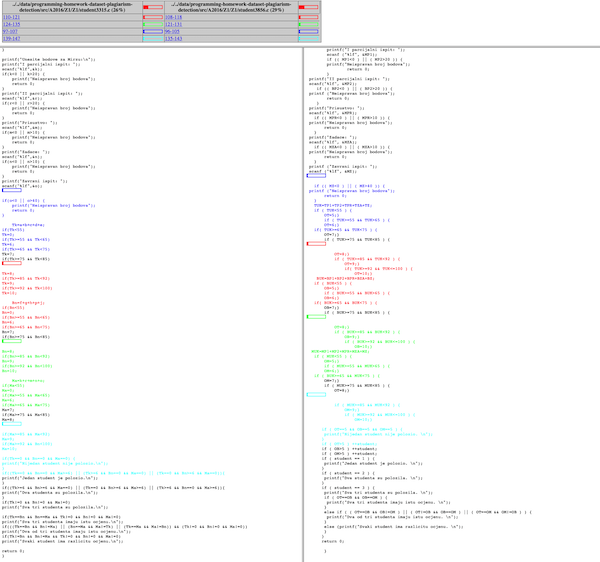
\includegraphics[scale=0.8]{images/MossExample.png}
\end{figure*}

\begin{table*}[t!]
\centering
\captionsetup{font=small}
\caption{\textsc{Levels Of Plagiarism}}
\label{table:plagiarization}
\resizebox{\textwidth}{!}{%
\begin{tabular}{lll}
\hline
\textbf{Level } & \textbf{ Attack Signatures}  & \textbf{Example} \\ \hline
1&Comment and whitespace modification& Removing all comments from given source code \\
\midrule
\addlinespace[0.5em]
2&\parbox{10cm}{Identifier modification (i.e., changing lexical name from one to another)} & Renaming all local variables \\
\midrule
\addlinespace[0.5em]
3&\parbox{10cm}{Component declaration relocation} & Moving all variable declarations to the beginning of main method \\
\midrule
\addlinespace[0.5em]
4& Method structure change & Replacing all method invocations with their respective invoked- method’s content \\
\midrule
\addlinespace[0.5em]
5&\parbox{10cm}{Program statement replacement (i.e., changing statements with other statements that share similar semantic yet different syntactic form) }& Replacing while statement with for statement \\
\midrule
\addlinespace[0.5em]
6&\parbox{10cm}{Logic change (i.e., changing statements with other statements that share no similarity in terms of syntactic and semantic form)} & \parbox{10cm}{Replacing an iterative traversal with the recursive one that generates similar result} \\
\midrule
\addlinespace[0.5em]
\end{tabular}%
}
\end{table*}

Karnalim VSM and LM Techniques Across Levels of Plagiarism
\begin{figure*}[ht!]
\centering
\begin{minipage}[b]{.4\textwidth}
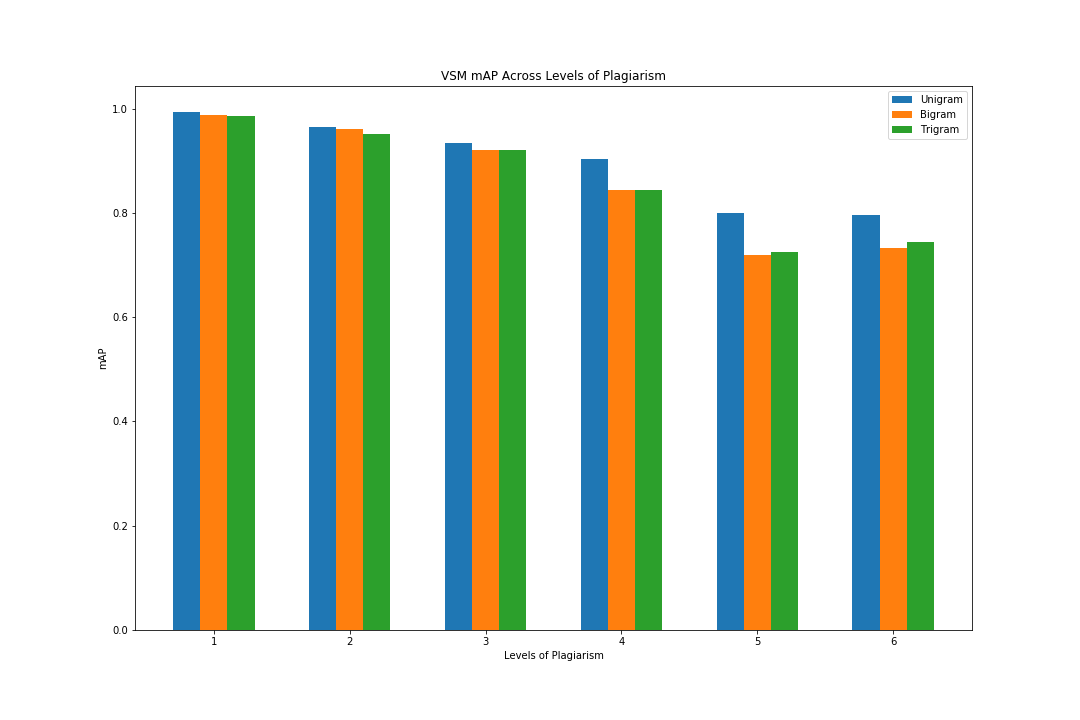
\includegraphics[width=1.0\textwidth]{images/VSM.png}
\caption{\textsc{VSM mAP Across Levels of Plagiarism}}\label{fig:vsm}
\end{minipage}\qquad
\begin{minipage}[b]{.4\textwidth}
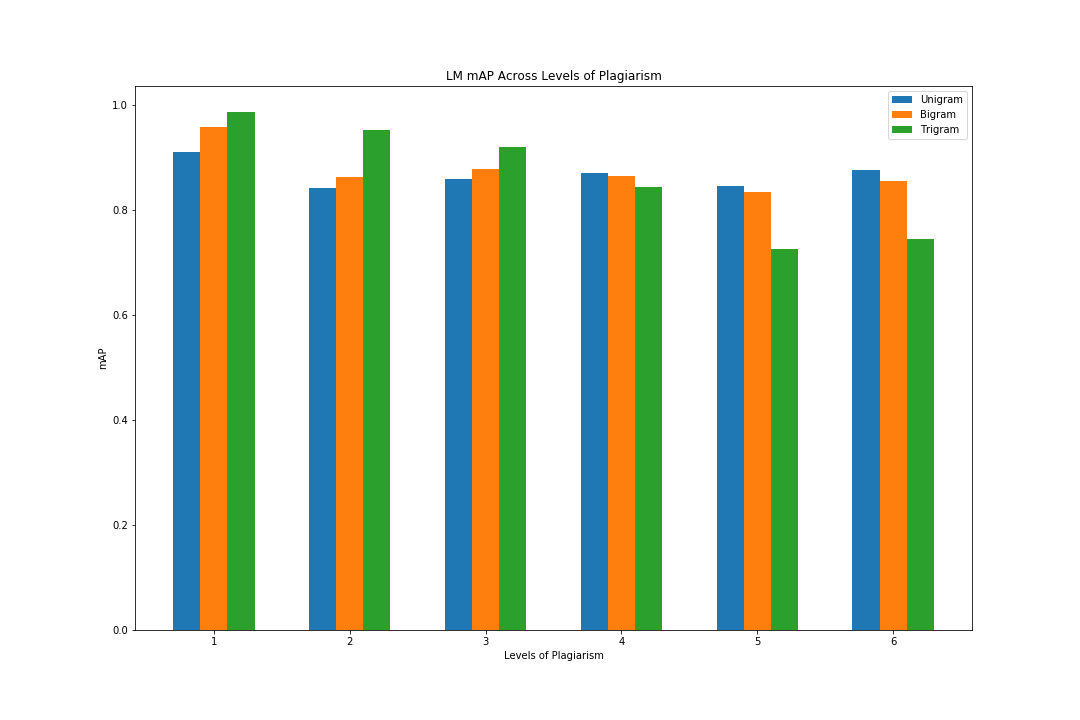
\includegraphics[width=1.0\textwidth]{images/LM.png}
\caption{\textsc{LM mAP Across Levels of Plagiarism}}\label{fig:lm}
\end{minipage}
\end{figure*}


\begin{figure*}[t!]
\centering
\caption{Error Analysis False Negative By BERT not in CodeBERT}
\label{fig:BERTnotinCodeBERT}
\centering
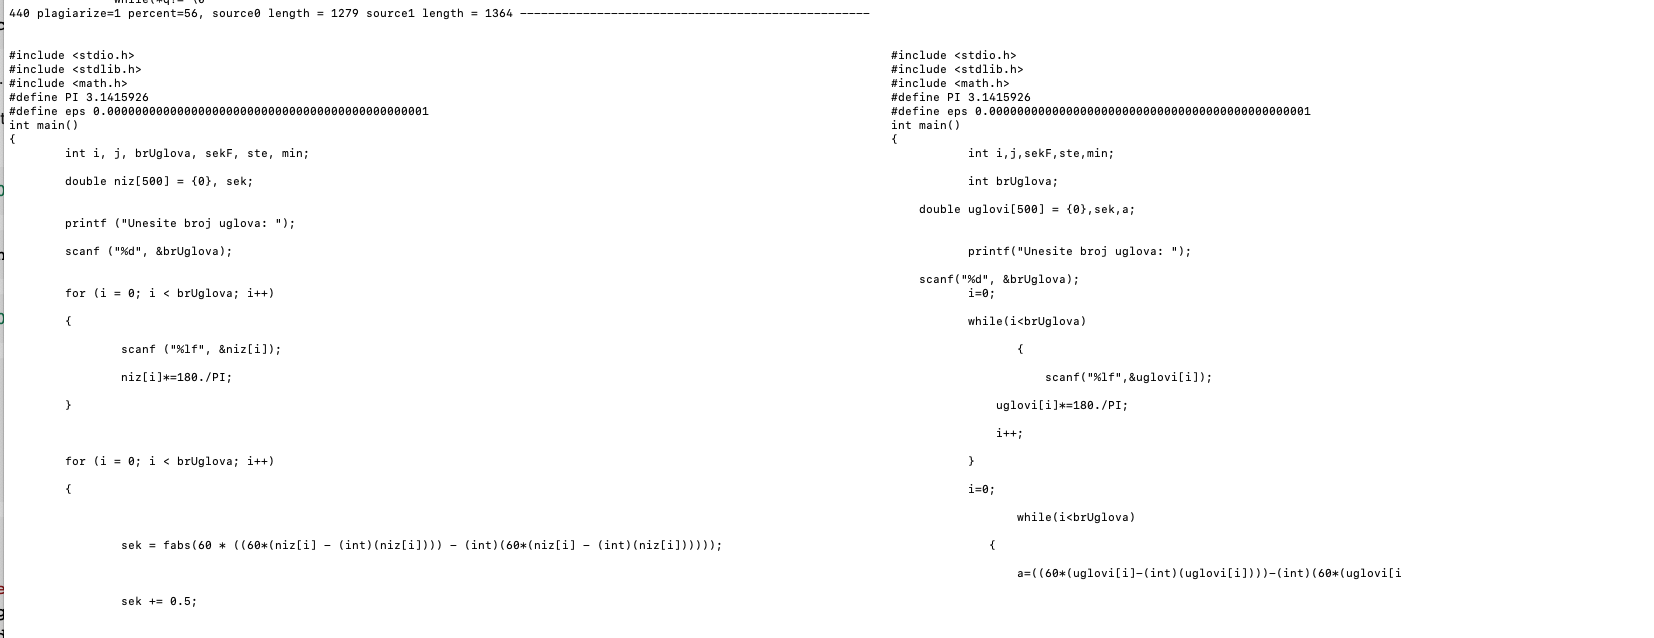
\includegraphics[scale=0.3]{images/FNinBERTnotinCodeBERT.png}
\end{figure*}

\begin{figure*}[t!]
\centering
\caption{Tokens Before and After ANTLR Preprocessing}
\label{fig:beforeandafterANTLR}
\centering
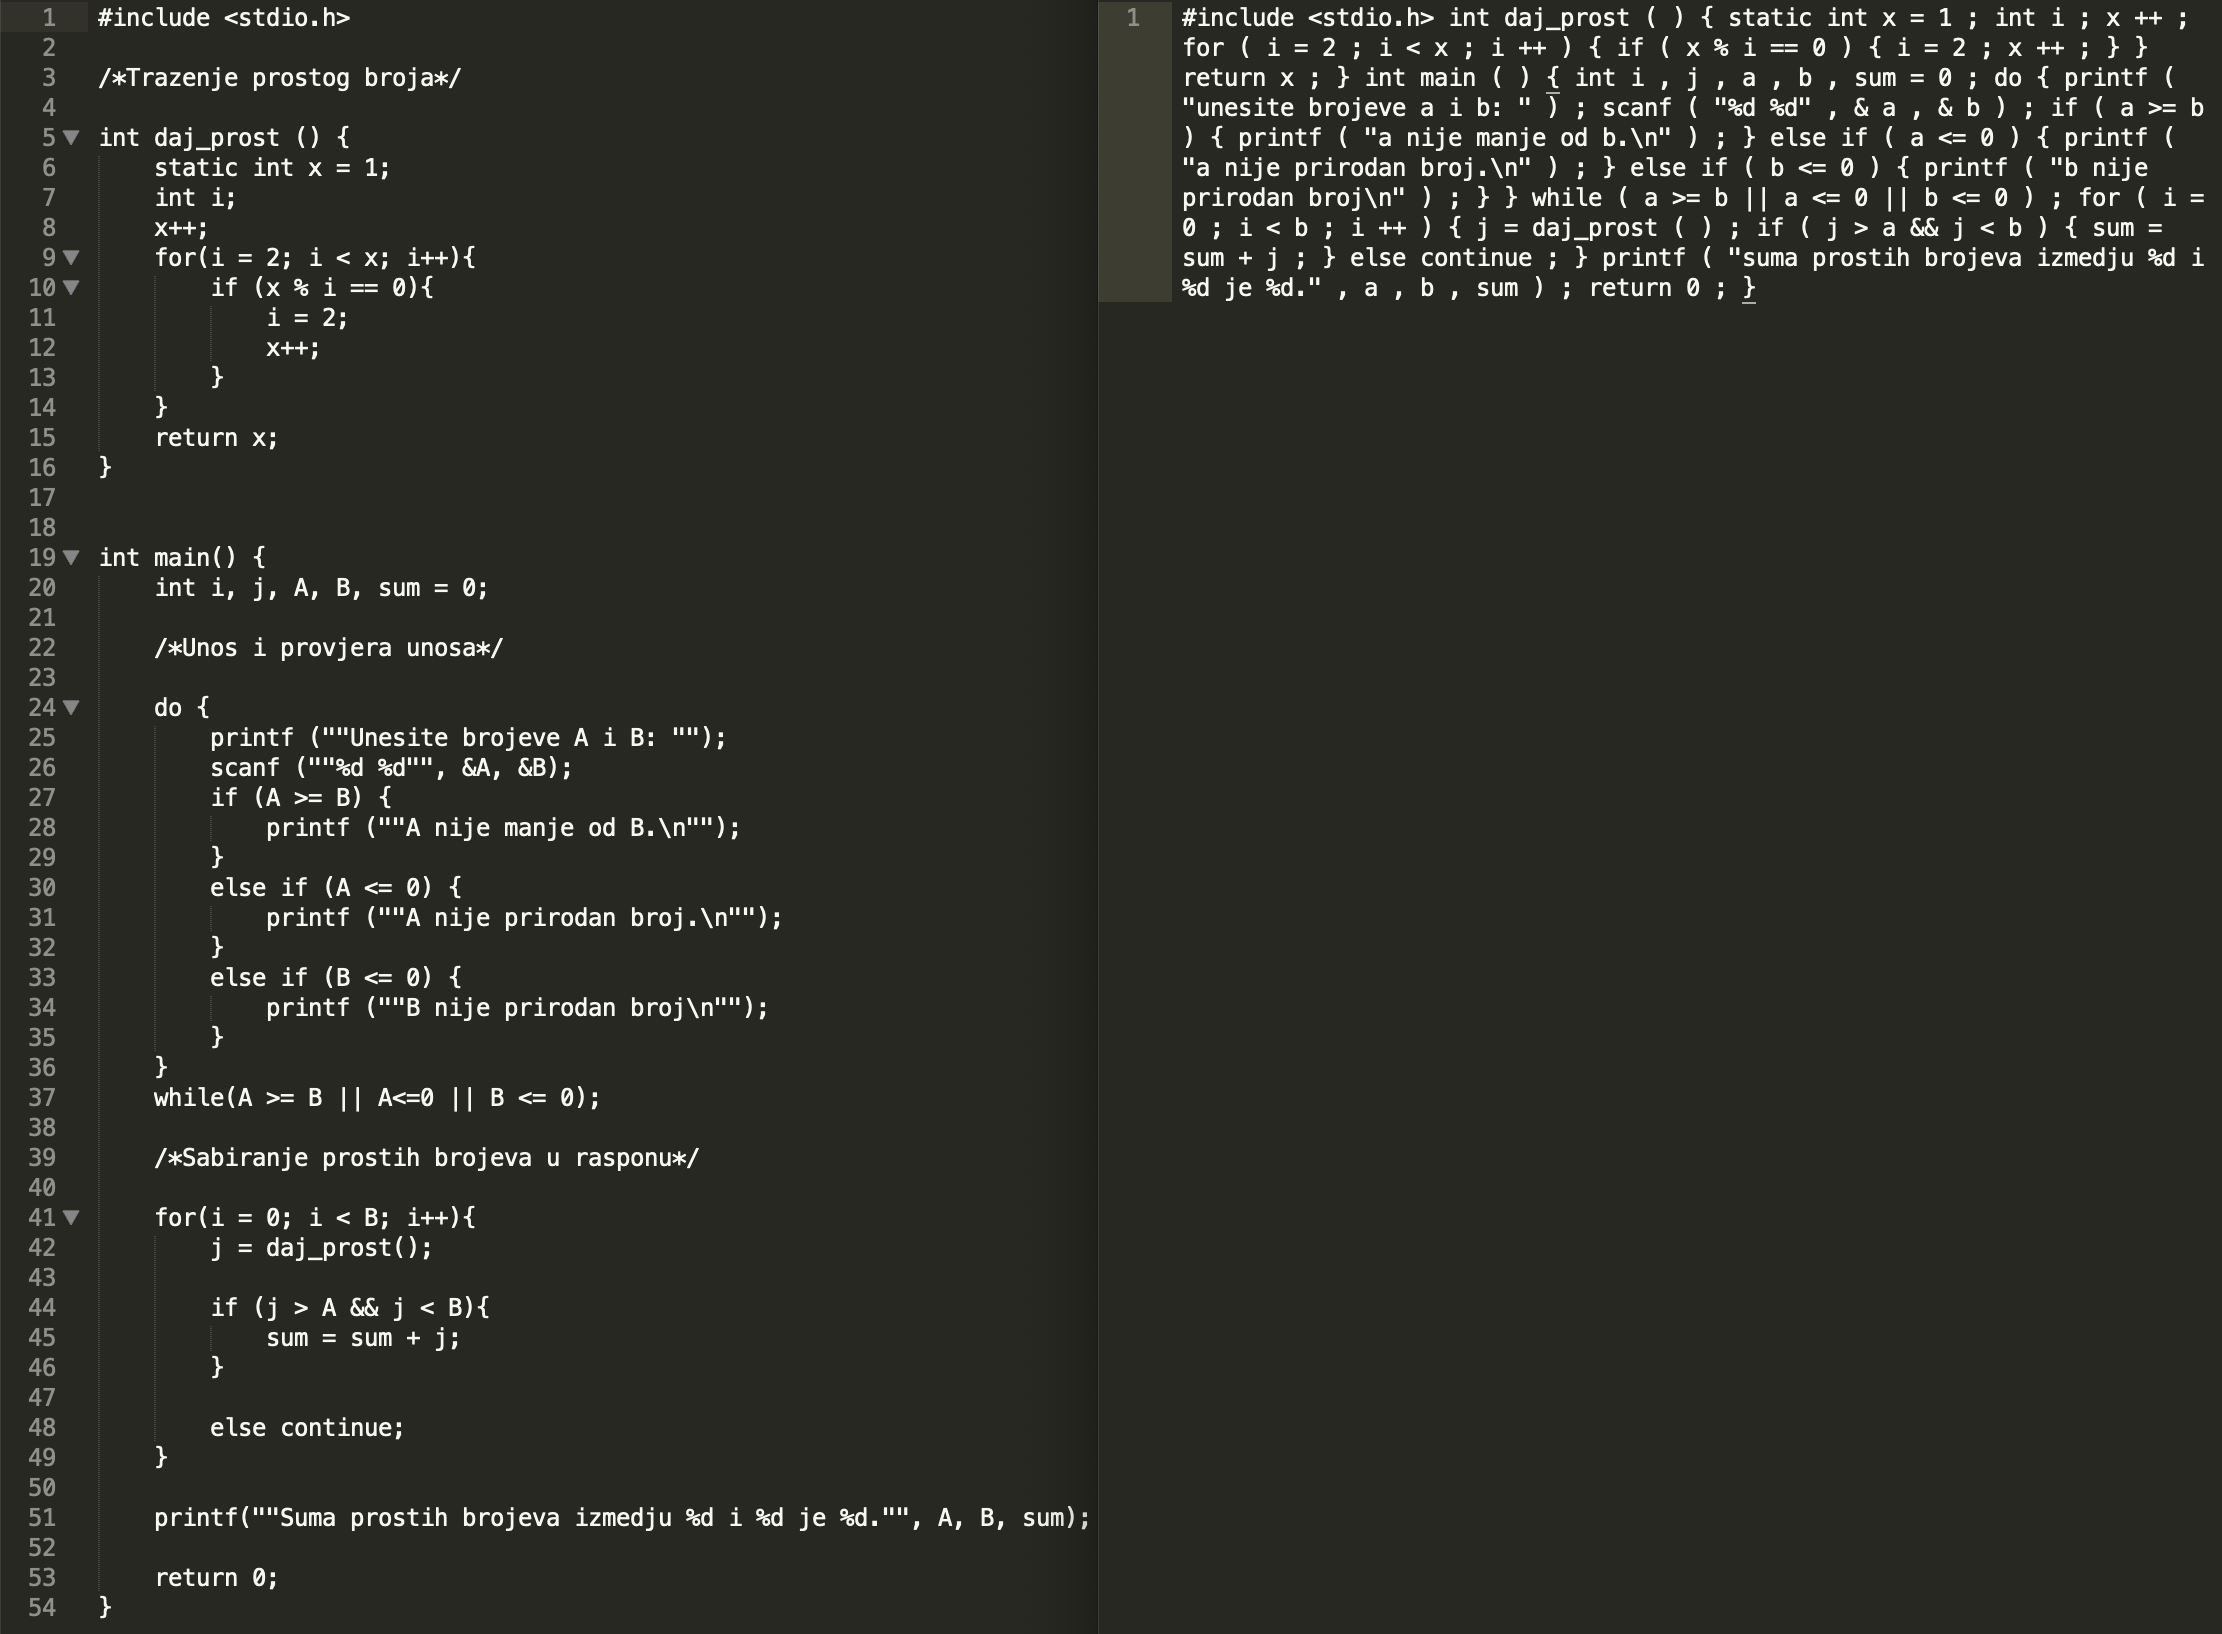
\includegraphics[scale=0.45]{images/tokens_comparison.png}
\end{figure*}

\begin{figure*}[t!]
\centering
\caption{BERT Tokenization vs CodeBERT Tokenization}
\label{fig:BERTtokenizationvsCodeBERTtokenization}
\centering
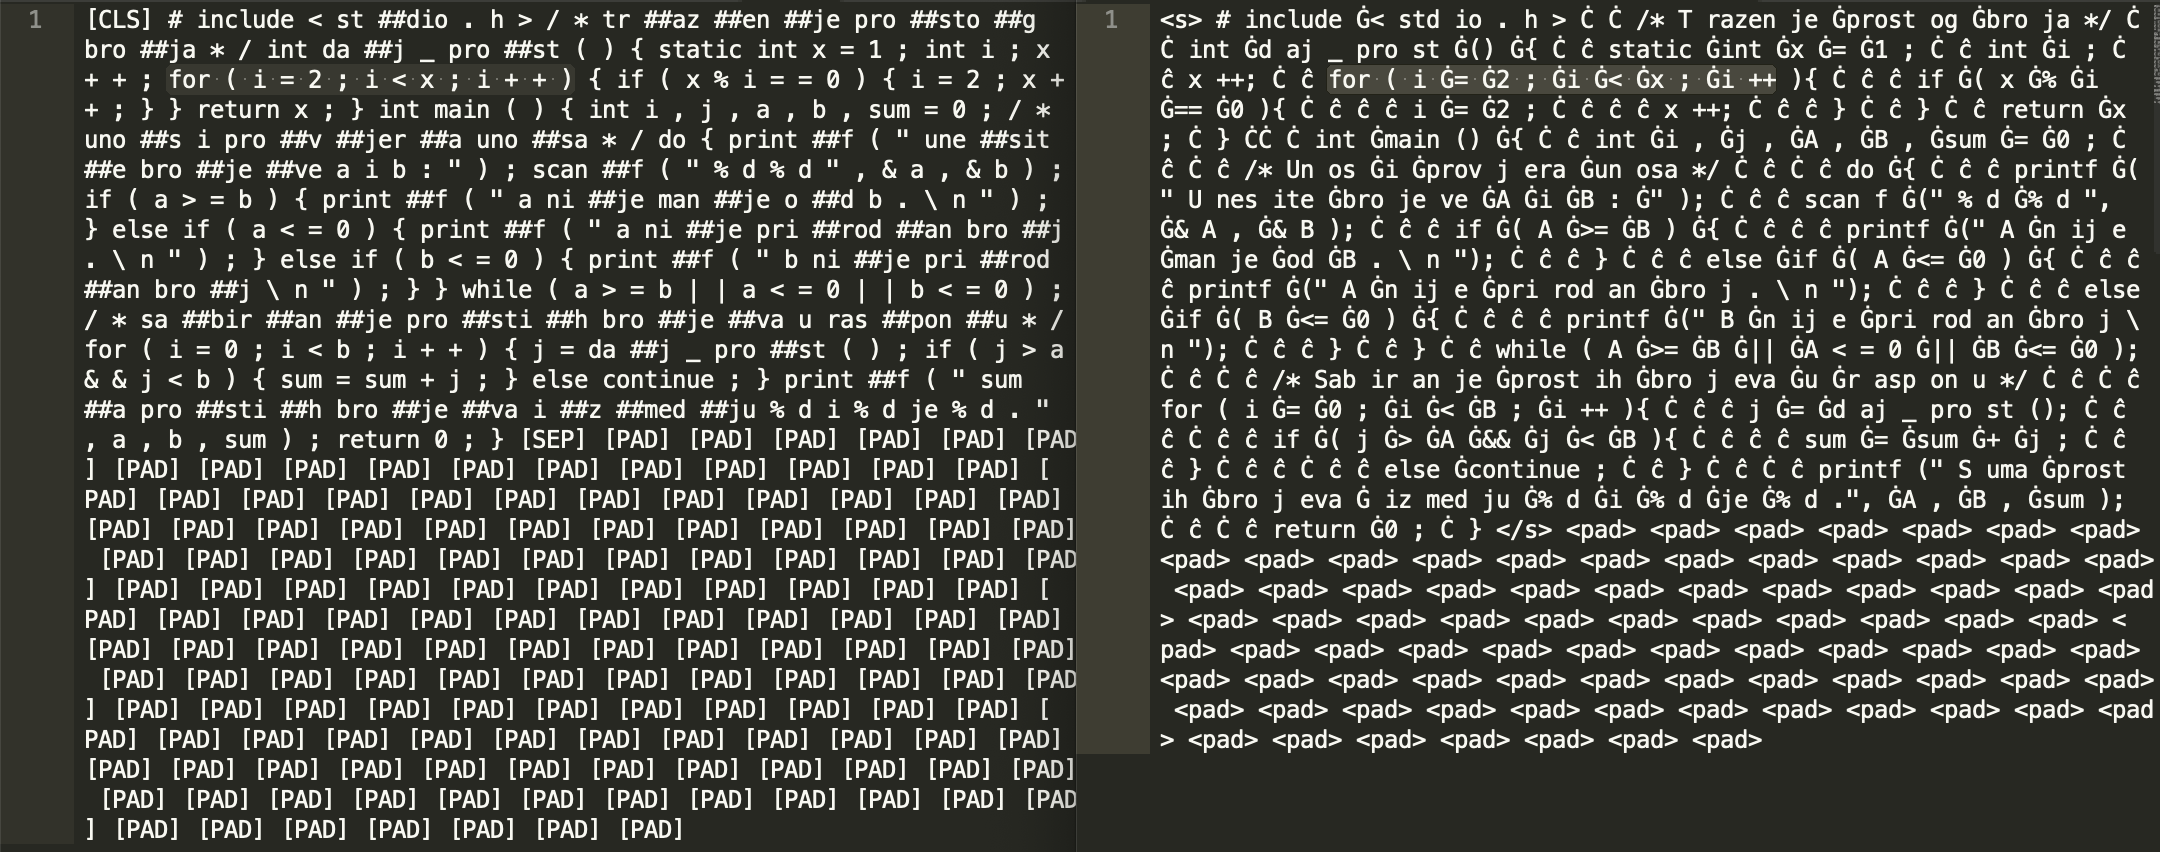
\includegraphics[scale=0.45]{images/tokenization_bert_vs_codebert_highlighted.png}
\end{figure*}


\begin{table*}[ht]
\centering
\captionsetup{font=small}
\caption{\textsc{Dataset Options}}
\label{table:datasetoptions}
\resizebox{\textwidth}{!}{%
\begin{tabular}{lll}
\hline
\textbf{Dataset} & \textbf{Features}  & \textbf{Challenges} \\ \hline
\parbox{7cm}{Programming Homework Dataset for Plagiarism Detection} & \parbox{7cm}{Actual Programming Assignments Of Varying Lengths. Reviewed by Professors and Challenge to students} & \parbox{7cm}{40,000 examples of C/C++ with only about 1,300 plagiarizations} \\
\midrule
\addlinespace[0.5em]
StaQC &\parbox{7cm}{Code Snippets in Python From Stack OverFlow. Over 148K Examples)} & \parbox{7cm}{Annotation with code and text pairs. No verification of plagiarism.}\\
\midrule
\addlinespace[0.5em]
IR-Plag &\parbox{7cm}{Canonically mapped based upon type of plagiarism} & \parbox{7cm}{Small size and only cover introductory programming.}\\
\midrule
\addlinespace[0.5em]
CodeXGlue &\parbox{7cm}{Clone Detection (POJ-104) Train 32K/Dev 8K/Test 12K examples spread amounst 64K problems} & \parbox{7cm}{Mostly small programming problems, not as variable as other programming assignments.}\\
\midrule
\addlinespace[0.5em]
\end{tabular}%
}
\end{table*}




































\end{document}






































\section{\large BLAH}

As an exploratory approach, we first attempted to replicate the Vector Space Model (VSM) and Language Model (LM) techniques from Karnalim, et. al. \cite{karnalim2019} on the Java source code plagiarism dataset they used. It's comprised of 105 non-plagiarized code files and 355 plagiarized code files across 7 original code files.[HARD TO FOLLOW PRIOR SENTENCE. '105...files and 355 files from...7 files'] We prepared both techniques by tokenizing the dataset using ANTLR (a customizable parsing tool) to parse the Java code files while ignoring whitespaces and comments. For the VSM based techniques, we first vectorized each file's token count with respect to the collection's token count. Then we compared the vector of each original code file to the vectors of its related files that were either plagiarized or not plagiarized to get cosine similarity values. For the LM based techniques, we compared the token count of each original code file against the token count of each of its related files and of the entire collection. We then used the similarity measure  Karnalim, et. al. \cite{karnalim2019} used to get the similarity value. This similarity value has a range from zero to positive infinity, and is larger the more similar the compared files are. For both techniques, we ended up ranking all the files based on the similarity values.

To assess their performance, we used the same method referenced by Karnalim, et. al. \cite{karnalim2019} that checks the mean average precision (mAP) based on file rankings where plagiarized files are expected to rank higher than non-plagiarized files.  On balance, our mAP values were similar to Karnalim et al. in the sense that we saw the best mAP values for the first level of plagiarism and progressively worse mAP values as we move up the levels of plagiarism.  We also attempted to use higher order ngrams, which yielded similar results compared to unigrams as seen in Figure 

We next attempted to use the VSM and LM based techniques on a portion of our main dataset consisting of 20044 source code files, of which 1296 files plagiarized off one another. Although the VSM based techniques consistently outperformed LM based techniques, neither technique attained mAP scores significantly greater than 0.5 regardless of the ngram.  At this point, we concluded these techniques did not perform well enough to pursue further.  Furthermore, we believe that assessing mAP by ranking plagiarized and non-plagiarized files did not seem as intuitive and comparable as other evaluation methods, especially when referenced against MOSS.  Therefore we decided to move on to other approaches.[I THINK THIS SECTION WOULD BE BEST SUMMARIZED BY ALBERT. MAYBE AIM FOR 1/2 THE CURRENT LENGTH. ONE VERY USEFUL BENEFIT OF THIS WORK WAS ANTLR WHICH ENDED UP BEING KEY TO OUR MAIN SOLUTION.]


% \begin{figure}[H]
% \centering
% 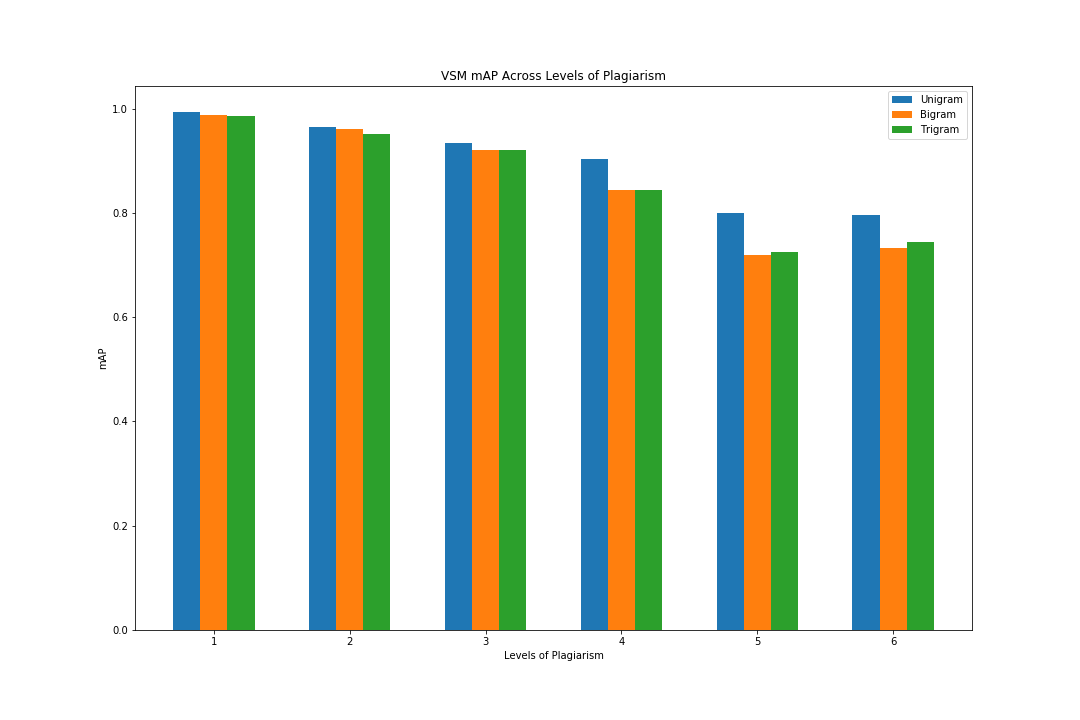
\includegraphics[width=0.45\textwidth]{images/VSM.png}
% \caption{\textsc{VSM mAP Across Levels of Plagiarism}}
% \label{fig:vsm}
% \end{figure}

% \begin{figure}[H]
% \centering
% 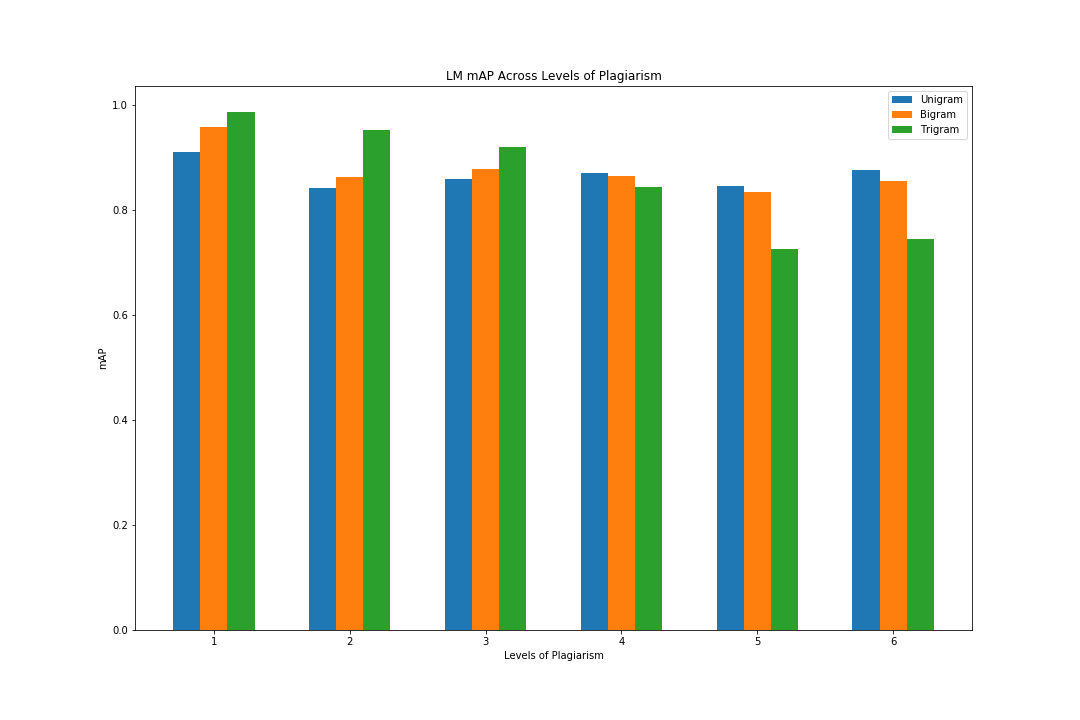
\includegraphics[width=0.45\textwidth]{images/LM.png}
% \caption{\textsc{LM mAP Across Levels of Plagiarism}}
% \label{fig:lm}
% \end{figure}


As mentioned in section 2, we used a generated dataset that used MOSS scores along with annotation from the Homework Plagiarization dataset. The result was that we could compare performance of MOSS versus the approaches we could take via experimentation. We will first look at how simple techniques like doing Sentence Embedding and Cosine Similarity can provide predictive power with respect to determining whether or not there was high similarity and plagiarism occurred.

Note that we have some very specific concerns when doing these experiments. Most of the source files are over 512 Tokens, the limitation for Models like Bert and CodeBert. This would mean that we would have to consider Models which can handle a larger number of tokens. We contemplated LongFormer, T5Large and BigBird. We did more experimentation with BigBird  and LonFormer for the learned models and the others, LongFormer and T5Large, using our Sentence-Transformer and cosine similarity with the embeddings (see Table \ref{table:mosscomparisons}  on page \pageref{table:mosscomparisons})




We started by looking at Cosine Similarity between embeddings generated by various models using MOSS as the metric for F1-score, along with Accuracy, Precision and Recall (Table \ref{table:mosscomparisons}  on page \pageref{table:mosscomparisons} ). Using this data we can see how each of these models would perform just based upon similarity for predicting plagiarism results. The data-set is balanced in terms of the minority class (code is similar and plagiarized).

It's fairly clear that while MOSS does well, with the highest F1-score, 0.7391 (meaning that we first start with looking at how similar documents are and we see the highest performance for MOSS at 97\% similarity between files) . When we look at all the other models using cosine similarity, we see little significant variation in F1-Score. 

We found this to be a counter-intuitive result. We expected LongFormer, T5Large and CodeBERT to have performed better than vanilla BERT for two reasons. BERT allows only 512 Tokens, and while CodeBERT has similar limitations, it is able to tokenize C code better than a BERT model. Similarly, LongFormer and T5Large would be able to handle at least up to 4K tokens and so could explain similarities better than BERT. Definitely quite surprising that none of these have better results that BERT.




After looking at the Cosine Similarity, it made sense to pursue answers to these questions using a BERT based model. We trained each of our models for 4 Epochs and used about 11K samples for training, about 3.5K for Validation and a similar amount for Testing. We used a BERT based Tokenizer (Roberta in the case of CodeBERT), and Models based upon Trainers for SequenceClassification. 

From the preliminary results, we see BERT again outperforming in terms of F1-Score (and surprising better with the model trained on Chinese), CodeBERT and even BigBird 2K,3K, and 4K and Longformer 4K. Why would this basic model outperform the more specialized Transformer models (see Table ~\ref{table:trainedmodels})? This is a mystery we'll investigate further. 










\begin{table*}[ht]
\centering
\captionsetup{font=small}
\caption{\textsc{Trained Model Performance}}
\fontsize{20}{24}\selectfont 
\label{table:trainedmodels}
\resizebox{\textwidth}{!}{%
\begin{tabular}{llllll}
\hline
\textbf{Model}   & \parbox{15cm}{Experiment Details} & \textbf{Accuracy} & \textbf{Precision}  & \textbf{Recall}  & \textbf{F1-Score}  \\ \hline
\parbox{10cm}{MOSS} & \parbox{15cm}{Code pairs, similarity, 50 setting for code common block. Evaluate at similarity above 73.1 \% to get max accuracy} & \parbox{7cm}{0.6970} & \parbox{7cm}{0.6840} & \parbox{7cm}{0.7325}  & \parbox{7cm}{0.7074}\\
\midrule
\hline
\parbox{10cm}{BERT}   & \parbox{15cm}{bert-base-uncased,512 tokens max ,learning rate 1e-5} & \parbox{7cm}{0.7833} & \parbox{7cm}{0.8032} & \parbox{7cm}{0.7505}  & \parbox{7cm}{0.7760}\\
\midrule 
\parbox{10cm}{BERT - Chinese Model}   & \parbox{15cm}{bert-base-chinese,512 tokens max,learning rate 1e-5}  & \parbox{7cm}{0.7676} & \parbox{7cm}{0.7460} & \parbox{7cm}{0.8114}  & \parbox{7cm}{0.7774}\\
\midrule 
\parbox{10cm}{BERT w/Whole Word}  & \parbox{15cm}{bert-large-uncased-whole-word-masking, 512 tokens,learning rate 1e-5} & \parbox{7cm}{0.8194} & \parbox{7cm}{\textbf{0.8809}} & \parbox{7cm}{0.7386}  & \parbox{7cm}{0.8035}\\
\midrule 
\parbox{10cm}{BERT w/Whole Word ANTLR}  & \parbox{15cm}{bert-large-uncased-whole-word-masking, ANTLR preprocessing remove whitespaces and comments, 512 tokens, learning rate 1e-5} & \parbox{7cm}{0.8195} & \parbox{7cm}{0.8041} & \parbox{7cm}{0.8449}  & \parbox{7cm}{0.8240}\\
\midrule 
\parbox{10cm}{CodeBERT}  & \parbox{15cm}{codebert-base,512 tokens, learning rate= 1e-5} & \parbox{7cm}{0.7845} & \parbox{7cm}{0.8144} & \parbox{7cm}{0.7367}   & \parbox{7cm}{0.7737}\\
\midrule 
\parbox{10cm}{CodeBERT ANTLR}  & \parbox{15cm}{codebert-base, ANTLR preprocessing remove whitespaces and comments, lower case tokens, 512 tokens, learning rate 5e-6} & \parbox{7cm}{\textbf{0.8634}} & \parbox{7cm}{0.8424} & \parbox{7cm}{\textbf{0.8940}}   & \parbox{7cm}{\textbf{0.8675}}\\
\midrule 
\parbox{10cm}{BigBird 1K}  & \parbox{15cm}{google/bigbird-roberta-base, 1K tokens, attention_type original_full, learning rate 1e-5}  & \parbox{7cm}{0.7369} & \parbox{7cm}{0.6992} & \parbox{7cm}{0.8318}  & \parbox{7cm}{0.7597}\\
\midrule 
\parbox{10cm}{BigBird 2K}  & \parbox{15cm}{google/bigbird-roberta-base, 2K tokens,learning rate 1e-5)}  & \parbox{7cm}{0.7585} & \parbox{7cm}{0.8369} & \parbox{7cm}{0.6421}  & \parbox{7cm}{0.7261}\\
\midrule 
\parbox{10cm}{Longformer 4K}  & \parbox{15cm}{allenai/longformer-base-4096, 4K tokens, learning rate 1e-5} & \parbox{7cm}{0.7140} & \parbox{7cm}{0.8322} & \parbox{7cm}{0.5361}  & \parbox{7cm}{0.6521}\\
\midrule
\addlinespace[0.5em]

\end{tabular}%
}
\end{table*}






To try and further improve our models, we analyzed some of the false negatives and false positives of our best models. One major issue we found was that whitespaces and comments took up a lot of tokens while yielding little to no predictive power in determining if a file was plagiarized or not. As a result, we brought back our ANTLR parsing to remove each file of its whitespaces and comments as a preprocessing step before training and evaluating. After rerunning our models with ANTLR preprocessing, we saw a noticeable improvement to the BERT Large model that uses whole word masking, but it was actually beaten by CodeBERT. In fact, CodeBERT with ANTLR preprocessing and lower cased tokens became our best model by far. We know that the preprocessing step effectively strips the document of all non-code elements and feeds more predictive code elements into the model than ever before. Since CodeBERT's tokenizer and model are trained on code elements, we theorize that it is able to make more use of this preprocessing to yield better predictive results, even without whole word masking.  








Our initial expectation was that using cosine similarity of embeddings would yield results similar to what MOSS was able to generate. When the results of the cosine similarities was averaged over the entire file, we felt that with unaltered model, we would still be able to have at least the same power as MOSS.

It soon became apparent that an untrained model was unable to fully address the layers of noise in the dataset. Our trained models were able to outperform pure MOSS based on the F1-score (except for Longformer 4K which requires further investigation). As we narrowed our focus on the reasons why our models performed so well, we looked at specific cases for CodeBERT and BERT against MOSS as seen in figure as we see in Table \ref{table:resultscomparison}, both BERT and CodBERT do really well on the True Negatives or correspondingly, MOSS has a much higher False positive count. Similarly MOSS has a higher False negative count when compared to both CodeBERT and BERT. When we look at CodeBERT and BERT , we see not a lot of difference in the True Negatives or specifically in the False Positives, but CodeBERT really shines in the True Positives, or more exactly vastly fewer False Negatives. We have detailed some of the reasons above, but we have included some specific examples in the appendix that highlight the power of preprocessing and a model trained on programming languages.

We saw CodeBERT perform significantly better than BERT at recognizing plagiarism from basic code replacements or structure changes.  For example, in Figure~\ref{fig:BERTnotinCodeBERT}, we see that CodeBERT was not fooled when a for loop was replaced with a while loop. Some other cases where CodeBERT demonstrated this ability include recognizing different formats for conditions (e.g. if else) and comparisons (e.g. >=<). Although CodeBERT was originally trained on many different languages, most to all of these languages share these basic code aspects.  Hence, we theorize that CodeBERT might recognize when these code structures have similar meanings, even if the tokens are different.






In addition, one challenge for the systems named above is that the code files being examined for similarity may contain between 4,000 and 10,000 tokens, far exceeding those systems' maximum input lengths of ~500 tokens. Our system has good predictability with a smaller number of tokens 512, but determining how to drive our models into much larger file sizes with the same or greater accuracy would be important, so perhaps using our Sentenc Transformer approach where we look at the entire file, but with our improved model could provide better results than even considering more work with LongT5\cite{guo}[up to 4K tokens], LongFormer\cite{beltagy}[up to 16K tokens] and PoolingFormer\cite{zhang}[up to 16K tokens], all of which might better help determine the similarity between entire documents. But the importance of having a model type such as CodeBERT, that is specifically trained on programming languages cannot be discounted.

In the end, we want to extend our models to perform as well a MOSS, which means being able to do comparisons on the order of a few tens of milliseconds, which at this point is not possible.






The models we developed when well trained, outperformed MOSS in predicting plagiarism where the connection between the plagiarized examples went beyond simple similarity of the code samples.
The dataset developers only looked at samples that were highly similar (using their toolset 99\%), yet even though this was necessary, it was not sufficient and the students involved where questioned directly to land on our plagiarized list. While MOSS failed to fully identify this X factor, a BERT based model was able to learn the key factors and outperform MOSS on this task on the test set.  Negatives, 





\subsection{\normalsize Key Learnings}

Proper preparation of the input dataset, and appyling masking appropriate to the task is a very useful tool irrespective of the model that is used. Powerful BERT based models when well trained on domain-specific datasets (such as with CodeBERT) can outperform industry standard tools such as MOSS even when looking at a relatively small amount of the source file data for the plagiarism detection task. The fact that these pretrained models require relatively little additional training on a small amount of the intended corpora to produce strong performance is an added benefit. Lastly, text preprocessing as a means to improve the signal to noise ratio provided a significant improvement in model performance. 